\documentclass[../main.tex]{subfiles}
\graphicspath{{\subfix{../figures/}}}
%
\begin{document}
%
\section{用例分析}
%
\subsection{需求分析}
通过对需求说明的详细分析, 我们可以得到:
此智慧食堂系统由用餐人员点餐、结算,以及食堂工作人员的配餐工作和查询分析组成。

其中的主要功能如下:
\begin{itemize}
  \item 用餐人员使用 APP 进行点餐:
    通过扫描餐桌上的二维码,用餐人员可以在APP中浏览菜品分类和具体菜品信息,并选择菜品和份数。点餐过程中可以随时终止本次点餐。APP上实时显示已选菜品的总份数和价格。
  \item 用餐人员结算:在点餐完成后,用餐人员可以进行结算,如果账户余额充足,则点餐成功;如果余额不足,则需要进行在线充值。
  \item 用餐人员取餐:在工作人员完成配餐后,用餐人员可以在食堂APP上看到配餐完成的提示,并且一体机会打印出一张含有餐位号和点餐人员ID的单据。用餐人员自行到取餐区取餐。
  \item 工作人员配餐:食堂工作人员使用带有触摸屏和打印机的一体机,在屏幕上显示分配给他的所有点餐记录,包括餐位号、菜品及其份数。工作人员按顺序进行配餐,点击开始按钮来为第一条点餐记录配餐,完成后点击完成按钮。
  \item 工作人员查询分析功能:可以通过该系统进行各种查询分析,如各菜品的受欢迎程度、食堂各时间段的用餐人数、平均点餐配餐时间、工作人员的工作量和累计收入等。
\end{itemize}
%
\subsection{用例描述}
\begin{itemize}
  \item 执行者: 顾客;
  \item 用例: 登录、点餐、在线支付等.
\end{itemize}
%
\begin{table}[H]
  \caption{顾客点餐-用例描述}
  \begin{center}
    \begin{tabular}[c]{l|l}
      \hline
      用例名称 & 顾客点餐 \\
      \hline
      执行者 & 顾客 \\
      \hline
      前置条件 & 已登录 \\
      \hline
      基本事件流 & \tabitem 顾客登录 \\
                 & \tabitem 顾客选择菜品 \\
                 & \tabitem 顾客在线支付 \\
                 & \tabitem 顾客点餐成功 \\
      \hline
      其他事件流 & \tabitem 顾客注册 \\
                 & \tabitem 顾客充值 \\
      \hline
      后置条件 & \tabitem 顾客点餐成功, 等待取餐 \\
               & \tabitem 顾客放弃点餐或余额不足进行充值后继续点餐. \\
      \hline
    \end{tabular}
  \end{center}
\end{table}
%
\begin{itemize}
  \item 执行者: 服务员;
  \item 用例: 登录、配餐、查询分析等.
\end{itemize}
%
\begin{table}[H]
  \caption{服务员配餐-用例描述}
  \begin{center}
    \begin{tabular}[c]{l|l}
      \hline
      用例名称 & 服务员配餐 \\
      \hline
      执行者 & 服务员 \\
      \hline
      前置条件 & 已登录 \\
      \hline
      基本事件流 & \tabitem 服务员登录  \\
                 & \tabitem 服务员为顾客配餐 \\
                 & \tabitem 服务员通过打印机打印单据 \\
                 & \tabitem 服务员处理点餐记录成功 \\
      \hline
      其他事件流 & \tabitem 服务员注册 \\
                 & \tabitem 服务员进行查询分析 \\
      \hline
      后置条件 & 服务员配餐成功, 处理下一条点餐记录(如果有的话) \\
      \hline
    \end{tabular}
  \end{center}
\end{table}
%
\subsection{用例图}
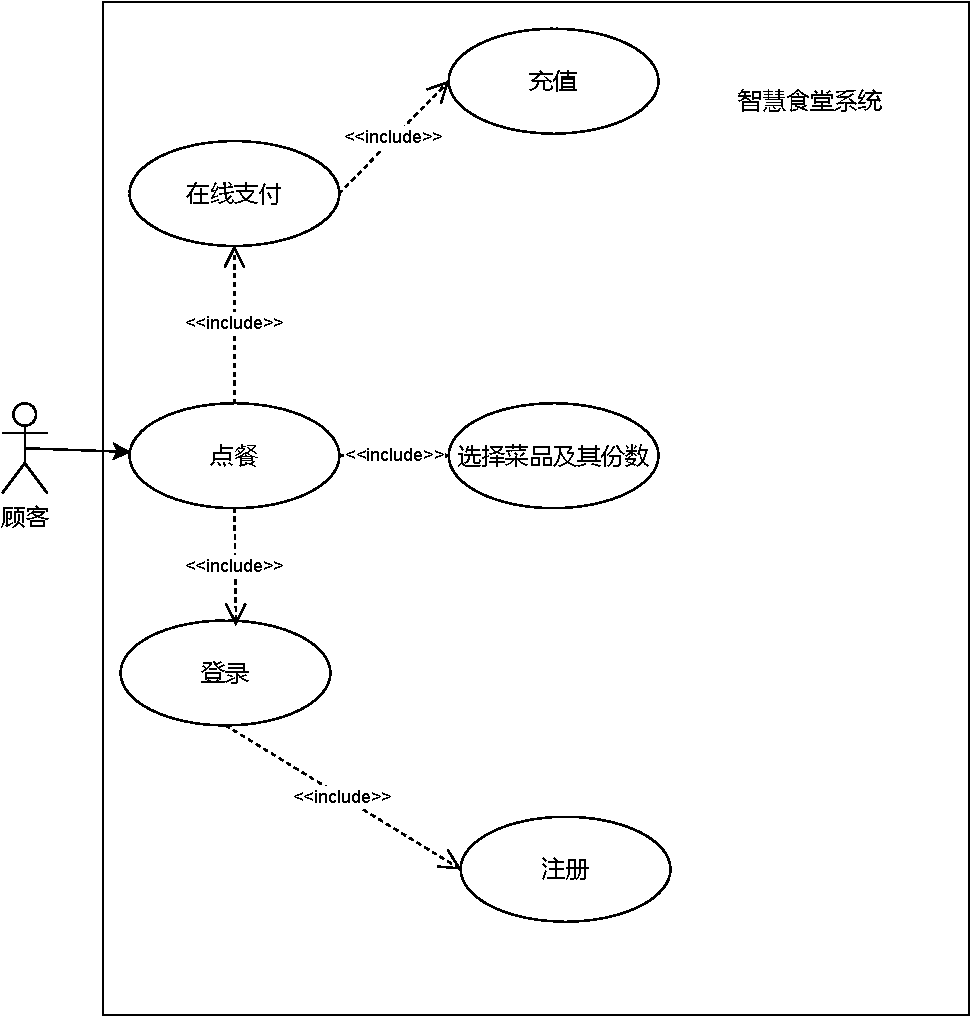
\includepdf[pages=1-1]{../resources/顾客用例图.pdf}
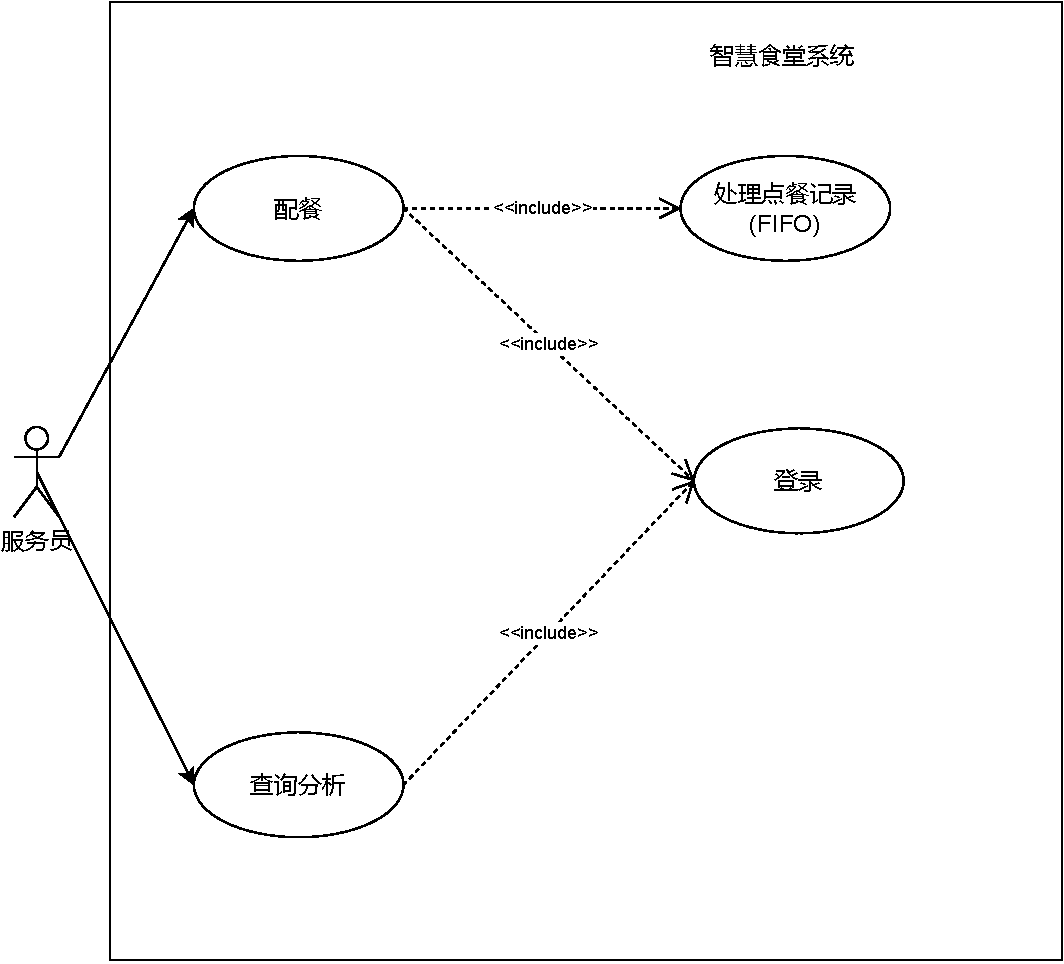
\includepdf[pages=1-1]{../resources/服务员用例图.pdf}
%
\end{document}
